\documentclass[12pt]{article}

\usepackage{times}
\usepackage{graphicx}
\usepackage{amsmath}
\usepackage{url}

\setlength{\textwidth}{6.5in}
\setlength{\textheight}{8.9in}
\setlength{\oddsidemargin}{0.0in}
\setlength{\topmargin}{0.05in}
\setlength{\headheight}{-0.05in}
\setlength{\headsep}{0.0in}

\newcommand{\indep}{\perp\!\!\!\perp}

\begin{document}

\begin{center}
{\bf CS 6300} \hfill {\large\bf HW09: VPI and HMMs \hfill {\bf Ryan Dalby} \hfill Due April 19, 2022}
\end{center}

\noindent
Please use the \LaTeX\ template to produce your writeups. See the
Homework Assignments page on the class website for details.  Hand in
via gradescope.

\section{Decision Networks and VPI}

A used car buyer can decide to carry out various tests with various
costs (e.g., kick the tires, take the car to a qualified mechanic) and
then, depending on the outcome of the tests, decide which car to buy.
We will assume that the buyer is deciding whether to buy the car and
that there is time to carry out at most one test which costs \$50 and
which can help to figure out the quality of the car.  A car can be in
good shape (of good quality Q = +q) or in bad shape (of bad quality
Q=-q), and the test might help to indicate what shape the car is in.
There are only two outcomes for the test T: pass (T=pass) or fail
(T=fail).  The car costs \$1,500, and its market value is \$2,000 if
it is in good shape; if not, \$700 in repairs will be needed to make
it in good shape.  The buyer's estimate is that the car has 70\%
chance of being in good shape.

\begin{enumerate}

\item  Draw the decision network that represents this problem.
\begin{center}
  \includegraphics[width=3in]{images/1a.png}
\end{center}

\begin{center}
  \begin{tabular}{|c|c|c|}
    \hline
    $U(\text{Buy}, Q)$ & $+q$ & $-q$ \\
    \hline
    $+\text{Buy}$ & $2000 - 1500 = 500$ & $2000 - (1500+700) = -200$ \\
    \hline
    $-\text{Buy}$ & $0$ & $0$ \\
    \hline
  \end{tabular}
\end{center}

\begin{center}
  \begin{tabular}{|c|c|}
    \hline
    $Q$ & $P(Q)$ \\
    \hline
    $+q$ & 0.70 \\
    \hline
    $-q$ & 0.30\\
    \hline
  \end{tabular}
\end{center}

\item  Calculate the expected net gain from buying the car, given no test.
\[
  EU(+\text{Buy}|\emptyset) = P(+q|\emptyset) U(+\text{Buy},+q) + P(-q|\emptyset) U(+\text{Buy},-q) 
\]

\[
  EU(+\text{Buy}|\emptyset) = P(+q) U(+\text{Buy},+q) + P(-q) U(+\text{Buy},-q) = (0.70)(500) + (0.30)(-200) = 290
\]

Also note that $\text{MEU}(\emptyset) = 290$ since $EU(-\text{Buy}|\emptyset) = 0$

\item Tests can be described by the probability that the car will pass
  or fail the test given that the car is in good or bad shape. We have
  the following information:

\begin{eqnarray*}
P(T = pass | Q = +q) &=&  0.9 \\
P(T = pass | Q = -q) &=&  0.2
\end{eqnarray*}

Calculate the probability that the car will pass (or fail) its test,
and then the probability that it is in good (bad) shape given each
possible test outcome.

\begin{center}
  \begin{tabular}{|c|c|c|}
    \hline
    $T$ & $Q$ & $P(T|Q)$ \\
    \hline
    $\text{Pass}$ & $+q$ & $0.9$ \\
    \hline
    $\text{Fail}$ & $+q$ & $0.1$ \\
    \hline
    $\text{Pass}$ & $-q$ & $0.2$ \\
    \hline
    $\text{Fail}$ & $-q$ & $0.8$ \\
    \hline
  \end{tabular}
\end{center}

\[
  P(T,Q) = P(T|Q)P(Q)
\]

\begin{center}
  \begin{tabular}{|c|c|c|}
    \hline
    $T$ & $Q$ & $P(T,Q)$ \\
    \hline
    $\text{Pass}$ & $+q$ & $(0.9)(0.7) = 0.63$ \\
    \hline
    $\text{Fail}$ & $+q$ & $(0.1)(0.7) = 0.07$ \\
    \hline
    $\text{Pass}$ & $-q$ & $(0.2)(0.3) = 0.06$ \\
    \hline
    $\text{Fail}$ & $-q$ & $(0.8)(0.3) = 0.24$ \\
    \hline
  \end{tabular}
\end{center}

\[
  P(T) = \sum_Q{P(T,Q)}
\]

\begin{center}
  \begin{tabular}{|c|c|}
    \hline
    $T$ & $P(T)$ \\
    \hline
    $\text{Pass}$ & $(0.63+0.06) = 0.69$ \\
    \hline
    $\text{Fail}$ & $(0.07+0.24) = 0.31$ \\
    \hline
  \end{tabular}
\end{center}

\[
  P(Q|T) = \frac{P(T,Q)}{P(T)}
\]

\begin{center}
  \begin{tabular}{|c|c|c|}
    \hline
    $T$ & $Q$ & $P(Q|T)$ \\
    \hline
    $\text{Pass}$ & $+q$ & $\frac{0.63}{0.69} = 0.913$ \\
    \hline
    $\text{Fail}$ & $+q$ & $\frac{0.07}{0.31} = 0.226$ \\
    \hline
    $\text{Pass}$ & $-q$ & $\frac{0.06}{0.69} = 0.0870$ \\
    \hline
    $\text{Fail}$ & $-q$ & $\frac{0.24}{0.31} = 0.774$ \\
    \hline
  \end{tabular}
\end{center}

\item Calculate the optimal decisions given either a pass or a fail,
  and their expected utilities.

  \[
    \text{MEU}(T) = \max_{\{+\text{Buy}, -\text{Buy}\}}{\sum_{Q}P(Q|T)U(Q|\text{Buy})}
  \]
  % \[
  %   \text{MEU}(T=\text{Pass}) = \max_{\{+\text{Buy}, -\text{Buy}\}}{P(+q|\text{Pass})U(+q|\text{Buy}) + P(-q|\text{Pass})U(-q|\text{Buy})}
  % \]
  \[
    \text{MEU}(T=\text{Pass}) = \max_{\{+\text{Buy}, -\text{Buy}\}}
    \begin{cases}
      P(+q|\text{Pass})U(+q|+\text{Buy}) + P(-q|\text{Pass})U(-q|+\text{Buy}) \\
      P(+q|\text{Pass})U(+q|-\text{Buy}) + P(-q|\text{Pass})U(-q|-\text{Buy}) \\
    \end{cases}
  \]
  \[
    \text{MEU}(T=\text{Pass}) = \max_{\{+\text{Buy}, -\text{Buy}\}}
    \begin{cases}
      (0.913)(500) + (0.0870)(-200) = 439.1 \\
      (0.913)(0) + (0.0870)(0) = 0 \\
    \end{cases}
    = 439.1
  \]
  Optimal decision for $\text{MEU}(T=\text{Pass})$ is $+\text{Buy}$ (Buy)


  \[
    \text{MEU}(T=\text{Fail}) = \max_{\{+\text{Buy}, -\text{Buy}\}}
    \begin{cases}
      P(+q|\text{Fail})U(+q|+\text{Buy}) + P(-q|\text{Fail})U(-q|+\text{Buy}) \\
      P(+q|\text{Fail})U(+q|-\text{Buy}) + P(-q|\text{Fail})U(-q|-\text{Buy}) \\
    \end{cases}
  \]
  \[
    \text{MEU}(T=\text{Fail}) = \max_{\{+\text{Buy}, -\text{Buy}\}}
    \begin{cases}
      (0.226)(500) + (0.774)(-200) = -41.8 \\
      (0.226)(0) + (0.774)(0) = 0 \\
    \end{cases}
    = -41.8
  \]
  Optimal decision for $\text{MEU}(T=\text{Fail})$ is $-\text{Buy}$ (Don't buy)

\item Calculate the value of (perfect) information of the test. Should
  the buyer pay for a test?

  \[
    \text{VPI}(T) = P(\text{Pass})(\text{MEU}(\text{Pass}) - \text{MEU}(\emptyset)) + P(\text{Fail})(\text{MEU}(\text{Fail}) - \text{MEU}(\emptyset))
  \]
  \[
    \text{VPI}(T) = (0.69)(439.1-290) + (0.31)(-41.8-290) = 0.021
  \]

  No, the buyer shouldn't pay \$50 for a test since $\text{VPI}(T) = \$ 0.021 < \$ 50$

\end{enumerate}

\clearpage

\section{HMMs}

You sometimes get colds, which make you sneeze. You also get
allergies, which make you sneeze. Sometimes you are well, which
doesn't make you sneeze (much). You decide to model the process using
the following HMM, with hidden states $X \in \{well, allergy, cold\}$ and
observations $E \in \{sneeze, quiet\}$:

\begin{center}
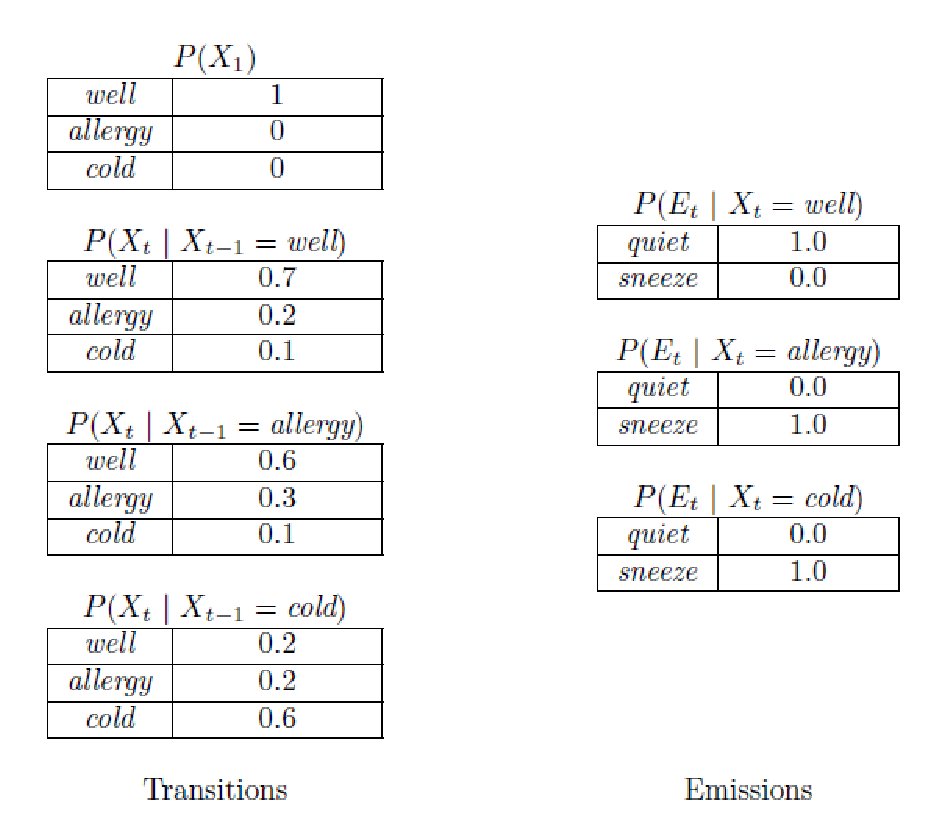
\includegraphics[height=4in]{sneeze.eps}
\end{center}

Note that colds are ``stickier'' in that you tend to have them for
multiple days, while allergies come and go on a quicker time
scale. However, allergies are more frequent. Assume that on the first
day, you are well.

Note for this problem, column vectors imply ``well'', ``allergy'', and ``cold'' for the unspecified state in the equation from top to bottom respectively.

\begin{enumerate}

\item What is the posterior distribution over your state on day 2
  ($X_2$) if $E_1 = quiet$, $E_2 = sneeze$?

  \[
    P(X_1|E_1=\text{quiet}) = 
    \begin{bmatrix}
      1 \\
      0 \\
      0 \\
    \end{bmatrix}
  \]

  This is equivalently represented as a table

  \begin{center}
    \begin{tabular}{|c|c|}
      \hline
      $X_1$ & $P(X_1|E_1=\text{quiet})$ \\
      \hline
      $\text{well}$ & 1 \\
      \hline
      $\text{allergy}$ & 0 \\
      \hline
      $\text{cold}$ & 0 \\
      \hline
    \end{tabular}
  \end{center}

  \[
    P(X_2|E_1=\text{quiet},E_2=\text{sneeze}) = \alpha P(\text{sneeze}|X_2) \sum_{X_1} {P(X_2|X_1) P(X_1|E_1=\text{quiet})}
  \]
  \[
    P(X_2|E_1=\text{quiet},E_2=\text{sneeze}) = 
    \alpha
    \begin{bmatrix}
      0 \\
      1.0 \\
      1.0 \\
    \end{bmatrix}
    (
    \begin{bmatrix}
      0.7 \\
      0.2 \\
      0.1 \\
    \end{bmatrix}
    (1)+
    \begin{bmatrix}
      0.6 \\
      0.3 \\
      0.1 \\
    \end{bmatrix}
    (0)+
    \begin{bmatrix}
      0.2 \\
      0.2 \\
      0.6 \\
    \end{bmatrix}
    (0)
    )=
    \begin{bmatrix}
      0 \\
      0.2 \\
      0.1 \\
    \end{bmatrix}
  \]
  Normalizing by $\alpha = \frac{1}{2/10 + 1/10} = \frac{10}{3}$
  \[
    P(X_2|E_1=\text{quiet},E_2=\text{sneeze}) =  
    \begin{bmatrix}
      0 \\
      2/3 \\
      1/3 \\
    \end{bmatrix}
  \]

  This is equivalently represented as a table

  \begin{center}
    \begin{tabular}{|c|c|}
      \hline
      $X_2$ & $P(X_2|E_1=\text{quiet},E_2=\text{sneeze})$ \\
      \hline
      $\text{well}$ & 0 \\
      \hline
      $\text{allergy}$ & $2/3$ \\
      \hline
      $\text{cold}$ & $1/3$ \\
      \hline
    \end{tabular}
  \end{center}

\item What is the posterior distribution over your state on day 3
  ($X_3$) if $E_1 = quiet$, $E_2 = sneeze$, $E_3 = sneeze$?

  \begin{multline*}
    P(X_3|E_1=\text{quiet},E_2=\text{sneeze},E_3=\text{sneeze}) = \\
    \alpha P(\text{sneeze}|X_3) \sum_{X_2} {P(X_3|X_2) P(X_2|E_1=\text{quiet},E_2=\text{sneeze})}
  \end{multline*}

  \begin{multline*}
    P(X_3|E_1=\text{quiet},E_2=\text{sneeze},E_3=\text{sneeze}) = \\
    \alpha
    \begin{bmatrix}
      0 \\
      1.0 \\
      1.0 \\
    \end{bmatrix}
    (
    \begin{bmatrix}
      0.7 \\
      0.2 \\
      0.1 \\
    \end{bmatrix}
    (0)+
    \begin{bmatrix}
      0.6 \\
      0.3 \\
      0.1 \\
    \end{bmatrix}
    (\frac{2}{3})+
    \begin{bmatrix}
      0.2 \\
      0.2 \\
      0.6 \\
    \end{bmatrix}
    (\frac{1}{3})
    )=
    \begin{bmatrix}
      0 \\
      4/15 \\
      4/15 \\
    \end{bmatrix}
  \end{multline*}
  Normalizing by $\alpha = \frac{1}{4/15+4/15} = \frac{15}{8}$
  \[
    P(X_3|E_1=\text{quiet},E_2=\text{sneeze},E_3=\text{sneeze}) =
    \begin{bmatrix}
      0 \\
      1/2 \\
      1/2 \\
    \end{bmatrix}
  \]

  This is equivalently represented as a table

  \begin{center}
    \begin{tabular}{|c|c|}
      \hline
      $X_3$ & $P(X_3|E_1=\text{quiet},E_2=\text{sneeze},E_3=\text{sneeze})$ \\
      \hline
      $\text{well}$ & 0 \\
      \hline
      $\text{allergy}$ & $1/2$ \\
      \hline
      $\text{cold}$ & $1/2$ \\
      \hline
    \end{tabular}
  \end{center}

\item What is the Viterbi (most likely) sequence for the observation
  sequence {\it quiet, sneeze, sneeze}?

  \[
    m_1(X_1) = P(\text{quiet}|X_1) P(X_1)
  \]
  
  \[
    m_1(X_1) =
    \begin{bmatrix}
      1 \\
      0 \\
      0 \\
    \end{bmatrix}
  \]

  This is equivalently represented as a table

  \begin{center}
    \begin{tabular}{|c|c|}
      \hline
      $X_1$ & $m_1(X_1)$ \\
      \hline
      $\text{well}$ & 1 \\
      \hline
      $\text{allergy}$ & 0 \\
      \hline
      $\text{cold}$ & 0 \\
      \hline
    \end{tabular}
  \end{center}

  \[
    m_2(X_2) = P(\text{sneeze}|X_2) \max_{X_1}{P(X_2|X_1) m_1(X_1)}
  \]
  \[
    m_2(X_2) = 
    \begin{bmatrix}
      0 \\
      1.0 \\
      1.0 \\
    \end{bmatrix}
    \max_{\text{well}, \text{allergy}, \text{cold}} 
    \begin{cases}
      \begin{bmatrix}
        0.7 \\
        0.2 \\
        0.1 \\
      \end{bmatrix} (1) = 
      \begin{bmatrix}
        0.7 \\
        0.2 \\
        0.1 \\
      \end{bmatrix}
      \\
      \begin{bmatrix}
        0.6 \\
        0.3 \\
        0.1 \\
      \end{bmatrix} (0) = 
      \begin{bmatrix}
        0 \\
        0 \\
        0 \\
      \end{bmatrix}
      \\
      \begin{bmatrix}
        0.2 \\
        0.2 \\
        0.6 \\
      \end{bmatrix} (0) =
      \begin{bmatrix}
        0 \\
        0 \\
        0 \\
      \end{bmatrix}
      \\
    \end{cases}
    =
    \begin{bmatrix}
      0 \\
      1.0 \\
      1.0 \\
    \end{bmatrix}
    \begin{bmatrix}
      0.7 \\
      0.2 \\
      0.1 \\
    \end{bmatrix}
    =
    \begin{bmatrix}
      0 \\
      0.2 \\
      0.1 \\
    \end{bmatrix}
  \]

  This is equivalently represented as a table

  \begin{center}
    \begin{tabular}{|c|c|}
      \hline
      $X_2$ & $m_2(X_2)$ \\
      \hline
      $\text{well}$ & 0 \\
      \hline
      $\text{allergy}$ & 0.2 \\
      \hline
      $\text{cold}$ & 0.1 \\
      \hline
    \end{tabular}
  \end{center}

  \[
    m_3(X_3) = P(\text{sneeze}|X_3) \max_{X_2}{P(X_3|X_2) m_2(X_2)}
  \]
  \[
    m_3(X_3) = 
    \begin{bmatrix}
      0 \\
      1.0 \\
      1.0 \\
    \end{bmatrix}
    \max_{\text{well}, \text{allergy}, \text{cold}} 
    \begin{cases}
      \begin{bmatrix}
        0.7 \\
        0.2 \\
        0.1 \\
      \end{bmatrix} (0) = 
      \begin{bmatrix}
        0 \\
        0 \\
        0 \\
      \end{bmatrix}
      \\
      \begin{bmatrix}
        0.6 \\
        0.3 \\
        0.1 \\
      \end{bmatrix} (0.2) = 
      \begin{bmatrix}
        0.12 \\
        0.06 \\
        0.02 \\
      \end{bmatrix}
      \\
      \begin{bmatrix}
        0.2 \\
        0.2 \\
        0.6 \\
      \end{bmatrix} (0.1) =
      \begin{bmatrix}
        0.02 \\
        0.02 \\
        0.06 \\
      \end{bmatrix}
      \\
    \end{cases}
    =
    \begin{bmatrix}
      0 \\
      1.0 \\
      1.0 \\
    \end{bmatrix}
    \begin{bmatrix}
      0.12 \\
      0.06 \\
      0.06 \\
    \end{bmatrix}
    =
    \begin{bmatrix}
      0 \\
      0.06 \\
      0.06 \\
    \end{bmatrix}
  \]

  This is equivalently represented as a table

  \begin{center}
    \begin{tabular}{|c|c|}
      \hline
      $X_3$ & $m_3(X_3)$ \\
      \hline
      $\text{well}$ & 0 \\
      \hline
      $\text{allergy}$ & 0.06 \\
      \hline
      $\text{cold}$ & 0.06 \\
      \hline
    \end{tabular}
  \end{center}

  There are two possible most likely sequences for this observation sequence depending on if the final element in the sequence is ``allergy'' or ``cold'' (either can be chosen since m values are the same):

  If ``allergy'' is chosen then the most likely sequence is ``well'' $->$ ``allergy'' $->$ ``allergy''.

  If ``cold'' is chosen then the most likely sequence is ``well'' $->$ ``cold'' $->$ ``cold''.

\end{enumerate}

\end{document}


